% Title: gl2ps_renderer figure
% Creator: GL2PS 1.4.2, (C) 1999-2020 C. Geuzaine
% For: Octave
% CreationDate: Mon Oct 31 14:18:23 2022
\setlength{\unitlength}{1pt}
\begin{picture}(0,0)
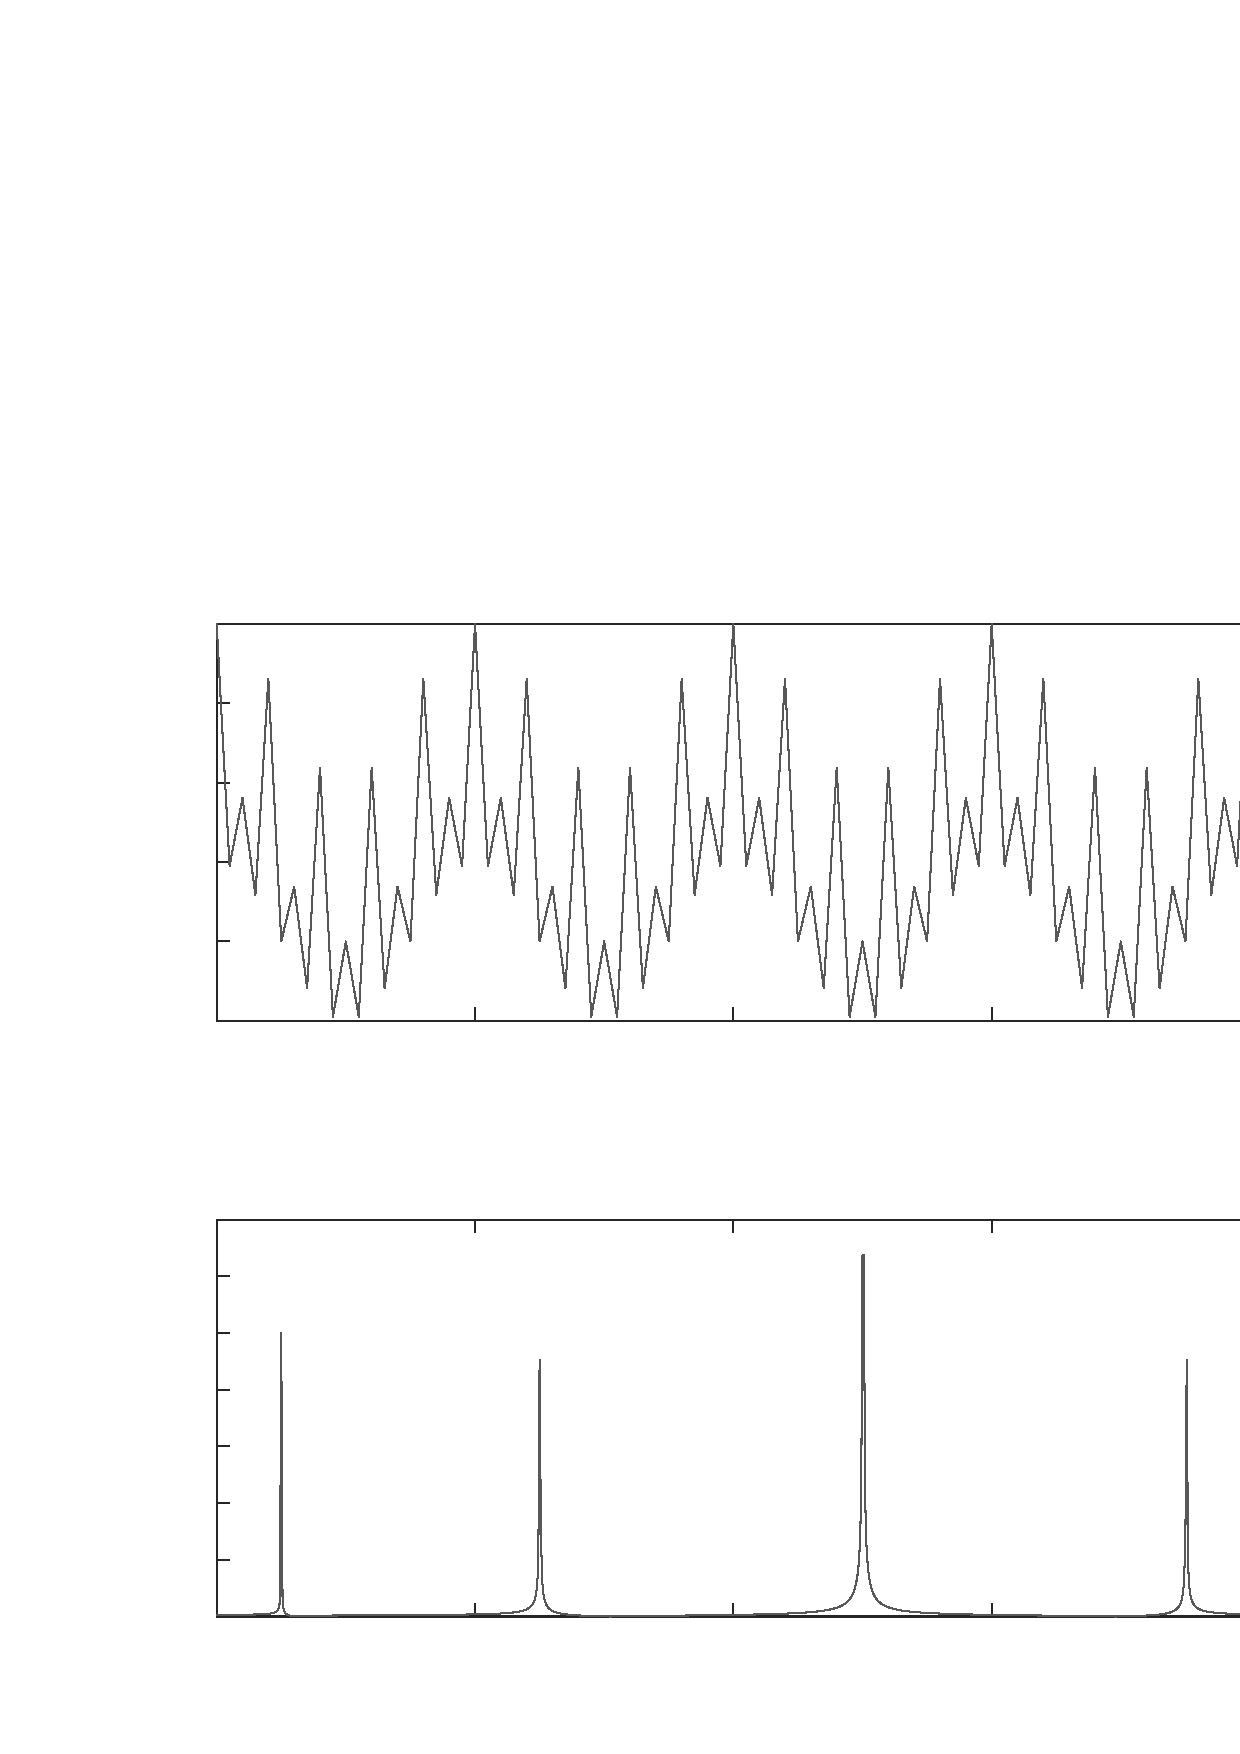
\includegraphics[scale=1]{octaves/cosineSumFT-inc}
\end{picture}%
\begin{picture}(800,600)(0,0)
\fontsize{13}{0}\selectfont\put(104,341.475){\makebox(0,0)[t]{\textcolor[rgb]{0.15,0.15,0.15}{{0}}}}
\fontsize{13}{0}\selectfont\put(228,341.475){\makebox(0,0)[t]{\textcolor[rgb]{0.15,0.15,0.15}{{0.2}}}}
\fontsize{13}{0}\selectfont\put(352,341.475){\makebox(0,0)[t]{\textcolor[rgb]{0.15,0.15,0.15}{{0.4}}}}
\fontsize{13}{0}\selectfont\put(476,341.475){\makebox(0,0)[t]{\textcolor[rgb]{0.15,0.15,0.15}{{0.6}}}}
\fontsize{13}{0}\selectfont\put(600,341.475){\makebox(0,0)[t]{\textcolor[rgb]{0.15,0.15,0.15}{{0.8}}}}
\fontsize{13}{0}\selectfont\put(724,341.475){\makebox(0,0)[t]{\textcolor[rgb]{0.15,0.15,0.15}{{1}}}}
\fontsize{13}{0}\selectfont\put(97.0525,351.924){\makebox(0,0)[r]{\textcolor[rgb]{0.15,0.15,0.15}{{-2}}}}
\fontsize{13}{0}\selectfont\put(97.0525,390.024){\makebox(0,0)[r]{\textcolor[rgb]{0.15,0.15,0.15}{{-1}}}}
\fontsize{13}{0}\selectfont\put(97.0525,428.124){\makebox(0,0)[r]{\textcolor[rgb]{0.15,0.15,0.15}{{0}}}}
\fontsize{13}{0}\selectfont\put(97.0525,466.224){\makebox(0,0)[r]{\textcolor[rgb]{0.15,0.15,0.15}{{1}}}}
\fontsize{13}{0}\selectfont\put(97.0525,504.324){\makebox(0,0)[r]{\textcolor[rgb]{0.15,0.15,0.15}{{2}}}}
\fontsize{13}{0}\selectfont\put(97.0525,542.424){\makebox(0,0)[r]{\textcolor[rgb]{0.15,0.15,0.15}{{3}}}}
\fontsize{15}{0}\selectfont\put(414,552.424){\makebox(0,0)[b]{\textcolor[rgb]{0,0,0}{{Sum of cosines}}}}
\fontsize{13}{0}\selectfont\put(104,55.5514){\makebox(0,0)[t]{\textcolor[rgb]{0.15,0.15,0.15}{{0}}}}
\fontsize{13}{0}\selectfont\put(228,55.5514){\makebox(0,0)[t]{\textcolor[rgb]{0.15,0.15,0.15}{{0.2}}}}
\fontsize{13}{0}\selectfont\put(352,55.5514){\makebox(0,0)[t]{\textcolor[rgb]{0.15,0.15,0.15}{{0.4}}}}
\fontsize{13}{0}\selectfont\put(476,55.5514){\makebox(0,0)[t]{\textcolor[rgb]{0.15,0.15,0.15}{{0.6}}}}
\fontsize{13}{0}\selectfont\put(600,55.5514){\makebox(0,0)[t]{\textcolor[rgb]{0.15,0.15,0.15}{{0.8}}}}
\fontsize{13}{0}\selectfont\put(724,55.5514){\makebox(0,0)[t]{\textcolor[rgb]{0.15,0.15,0.15}{{1}}}}
\fontsize{13}{0}\selectfont\put(97.0525,66){\makebox(0,0)[r]{\textcolor[rgb]{0.15,0.15,0.15}{{0}}}}
\fontsize{13}{0}\selectfont\put(97.0525,93.2143){\makebox(0,0)[r]{\textcolor[rgb]{0.15,0.15,0.15}{{100}}}}
\fontsize{13}{0}\selectfont\put(97.0525,120.429){\makebox(0,0)[r]{\textcolor[rgb]{0.15,0.15,0.15}{{200}}}}
\fontsize{13}{0}\selectfont\put(97.0525,147.643){\makebox(0,0)[r]{\textcolor[rgb]{0.15,0.15,0.15}{{300}}}}
\fontsize{13}{0}\selectfont\put(97.0525,174.857){\makebox(0,0)[r]{\textcolor[rgb]{0.15,0.15,0.15}{{400}}}}
\fontsize{13}{0}\selectfont\put(97.0525,202.071){\makebox(0,0)[r]{\textcolor[rgb]{0.15,0.15,0.15}{{500}}}}
\fontsize{13}{0}\selectfont\put(97.0525,229.286){\makebox(0,0)[r]{\textcolor[rgb]{0.15,0.15,0.15}{{600}}}}
\fontsize{13}{0}\selectfont\put(97.0525,256.5){\makebox(0,0)[r]{\textcolor[rgb]{0.15,0.15,0.15}{{700}}}}
\fontsize{15}{0}\selectfont\put(414,266.5){\makebox(0,0)[b]{\textcolor[rgb]{0,0,0}{{Fourier Transform}}}}
\end{picture}
